\chapter{Introduction}




\section{The Goal Structuring Notation}

The Goal Structuring Notation (GSN) is a graphical argumentation notation,
which aims to allow the communication of logical arguments more clearly, and in a more structured way, than prose.

\citet{kelly2004goal} present the GSN as ``a safety agrument notation'',
referring to \emph{safety cases} which are used to argue that safety-critical systems are sufficiently safe,
particularly in the aerospace, railway and defence industries.
They observe that
``Not all engineers responsible for producing safety cases write clear and
well-structured English'',
and that
``cross-references \ldots can be awkward and can disrupt the flow of the main argument.'' 
The GSN is ``a structured technique that has been developed to address the
problems of clearly expressing and presenting safety argument.''

\citet{Habli:2006:PPC:1183088.1183090} list some of the applications of the GSN up to \citeyear{Habli:2006:PPC:1183088.1183090}:

\begin{itemize*}
  \item{Eurofighter Aircraft Avionics Safety Justification}
  \item{Hawk Aircraft Safety Justification}
  \item{U.K. Ministry of Defence Site Safety Justifications}
  \item{U.K. Dorset Coast Railway Re-signalling Safety Justification}
  \item{Submarine Propulsion Safety Justifications}
  \item{Safety Justification of UK Military Air Traffic Management Systems}
  \item{London Underground Jubilee Line Extension Safety Justification}
  \item{Swedish Air Traffic Control Applications}
  \item{Rolls-Royce Trent Engine Control Systems Safety Arguments}
\end{itemize*}

There is also evidence of the GSN being used for presenting other kinds of logical argument:
for example,
arguing the security of a system \cite{plop},
and validating computer simulations of biological models \cite{insilico} \todo{space or not? (!)} \cite{royal}. The field of argumentation is broad \ldots \todo{potential use by lawyers, philosophers?}

GSN arguments are directed, multivariate, hierarchical, two dimensional graphs.
The nodes are made up of the following types of element:

\begin{description}

  \item[\tikz{ \draw rectangle (4ex,2ex); } Goal/claim ]
    a statement that can be assessed to be true or false

  \item[\tikz{ \draw (0,0) -- (3.5ex,0) -- (4ex,2ex) -- (0.5ex,2ex) -- (0,0); } Strategy]
    a course of action that should be taken in order to validate the claim
  
  \item[\tikz{ \draw circle (1ex); } Solution]
      often the name of another document that should be produced in order to validate [?] the argument 

  \item[\tikz{ \draw [rounded corners=1ex] rectangle (4ex,2ex); } Context]
    often the name of another document

  \item[\tikz{ \draw ellipse (2ex and 1ex); } Assumption]
    an assumption

  \item[\tikz{\draw [baseline=-0.5ex] ellipse (2ex and 1ex);} Justification]

\end{description}

Edges connect these elements together, forming an overall ``goal structure''. 

\begin{figure}
  \centering
  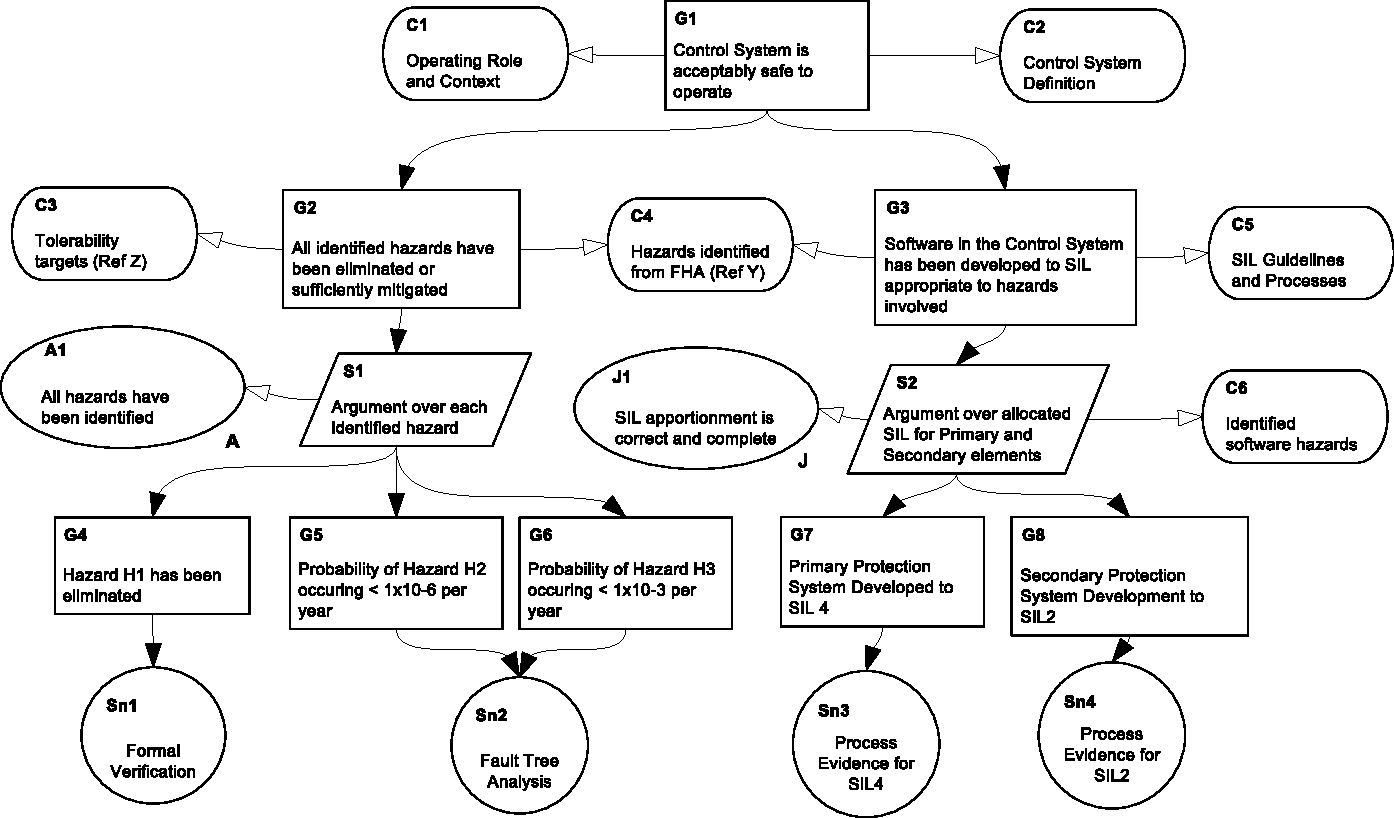
\includegraphics[width=\textwidth]{example_argument.pdf}
  \caption{An example GSN argument, about a safety case,
    from the GSN specification \cite{gsnstandard}}
  \label{fig:crampedex1}
\end{figure}




\section{Artoo}

Artoo (Argumentation Tool) is a tool for drawing graph[ical?] structures, specifically using the GSN syntax. It was developed by Paul Andrews at the York Computational Immunology Lab, and [is therefore particularly well-suited to?] using the GSN to argue about biological simulations (for example, it allows arguments to be ``unfinished'') as \citet{royal} do in a paper which introduces both Artoo and the use of the argumentation (specifically using the GSN) for this \ldots \todo{a bit clumsy?}

Artoo is a single-page, client-side web application, written in JavaScript, and runs in recent versions of most popular web browsers. Arguents are displayed as [embedded in the web page] Scalable Vector Graphics (SVG) documents, can be stored as XML documents (containing all information about arguments' structure, semantics and layout), and can be exported as bitmap images.

\ldots

Artoo is available for free under a GNU GPLv3 licence.
This means that anyone can use it and modify it, within the terms of the license.
Other tools also exist for drawing GSN arguments, but they are typically commercial and closed-source, and emphasise the use of the GSN for presenting safety arguments.
Examples include Dependable Computing's Argument Editor\footnote{\url{http://www.dependablecomputing.com/tools/index.html}} \ldots

\begin{figure}
  \centering
  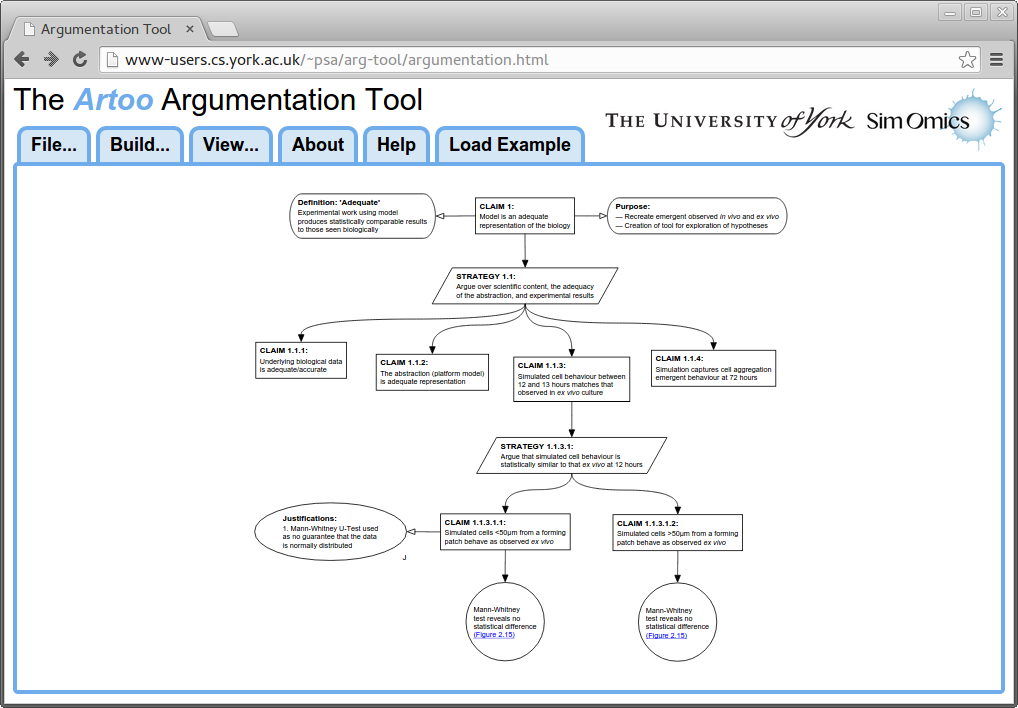
\includegraphics[width=\textwidth]{graphics/artoo_screenshot.png}
  \caption{The Artoo tool, displaying an argument}
\end{figure}

\section{Automatic layout of GSN arguments in the Artoo tool}

Currently, users of Artoo have full control over the layout of arguments they draw, and have to position each node on the infinite canvas using a pointing device.
(Edges are drawn automatically, based on connections defined \todo{?} by the user.)
Clearly, this becomes difficult to manage for larger arguments, and is made harder by the absence of features such as ``snap to grid'' \todo{cite somehow?}.
Furthermore, users sometimes perform manual layout badly -- for example, the dense layout of the argument shown in figure~\ref{fig:crampedex1} makes its structure hard to discern [hides/masks its structure?] \ldots \todo{needs more something?}.

For these reasons, graph drawing tools often include automatic layout features. Examples include, Dependable Computing's Argument Editor \todo{see footnote 1?} \ldots

This project aims to add an automatic layout feature to Artoo.
How this will be exposed to the user is still to be determined. 
The process will involve researching and implementing various graph layout algorithms,
and testing them [in a structured, repeatable way] in order to compare them. 

\subsection{Problem definition}

Typically, a graph layout algorithm takes as its inputs a set of nodes and a set of edges, [and outputs \ldots] [not a controversial statement but might cite].
In the case of a GSN argument, there is additional information associated with the input graph:

\begin{itemize}
  \item
    Each node has a width and a height, whereas in the simplest model of a graph nodes are single points. \todo{,?}
  \item
    There are various types of node and edge, and the type of a node should influence where it is placed. Specifically: goals, stategies and solutions should be treated differently to context, assumption and justification elements.
    \begin{itemize}
    \item The GSN specification's layout guidance \citep[section~2.2, pp.~26--27]{gsnstandard} recommends that parent and child goals, stategies and solutions are placed above and below each other; context, assumption and justification elements should be placed to the left and right of their parents (helping to alleviate the problem of cross-references disrupting the flow of arguments) \todo{slightly too much detail here, move to later section?}.
    \end{itemize}
\end{itemize}

A structured, repeatable way of assessing and comparing graph layout algorithms will be produced. 

\ldots

\subsection{this probably belongs later:}

Artoo also allows the drawing of invalid GSN argments ...
if the graph layout [thing] is to be executed every time the graph is edited, then it must accept these .
If the algorithm [is exposed to the user by a] button, then there is the poissibility of checking 

Already, Artoo only works a limited set of web browsers: recent versions of \ldots
The features added in this project will not interact with the browser in any new way -- only needing to change the position of nodes, using methods already in the code -- it is very unlikely that there will be any problems \ldots

\subsection{method}


  \begin{enumerate}
    \item
      \begin{itemize}
      \item ,
    \end{itemize}
  \end{enumerate}
